\documentclass[11pt]{article}
\usepackage[scheme=plain]{ctex}
\usepackage[a4paper]{geometry}
\geometry{left=2.0cm,right=2.0cm,top=2.5cm,bottom=2.5cm}

\usepackage{comment}
\usepackage{booktabs}
\usepackage{graphicx}
\usepackage{diagbox}
\usepackage{amsmath,amsfonts,graphicx,amssymb,bm,amsthm}
%\usepackage{algorithm,algorithmicx}
\usepackage[ruled]{algorithm2e}
\usepackage[noend]{algpseudocode}
\usepackage{fancyhdr}
\usepackage{tikz}
\usepackage{graphicx}
\usetikzlibrary{arrows,automata}
\usepackage{hyperref}
\hypersetup{
	colorlinks=true,
	linkcolor=blue,
	filecolor=blue,      
	urlcolor=blue,
	citecolor=cyan,
}			

\setlength{\headheight}{14pt}
\setlength{\parindent}{0 in}
\setlength{\parskip}{0.5 em}

\newtheorem{theorem}{Theorem}
\newtheorem{lemma}[theorem]{Lemma}
\newtheorem{proposition}[theorem]{Proposition}
\newtheorem{claim}[theorem]{Claim}
\newtheorem{corollary}[theorem]{Corollary}
\newtheorem{definition}[theorem]{Definition}
\newtheorem*{definition*}{Definition}

\newenvironment{problem}[2][Problem]{\begin{trivlist}
\item[\hskip \labelsep {\bfseries #1}\hskip \labelsep {\bfseries #2.}]}{\hfill$\blacktriangleleft$\end{trivlist}}
\newenvironment{answer}[1][Answer]{\begin{trivlist}
\item[\hskip \labelsep {\bfseries #1.}\hskip \labelsep]}{\hfill$\lhd$\end{trivlist}}

\newcommand\E{\mathbb{E}}
\newcommand\per{\mathrm{per}}
\newcommand\dd{\mathrm{d}}
\newcommand\e{\mathrm{e}}

\title{Homework \#1}
\usetikzlibrary{positioning}

\begin{document}

\pagestyle{fancy}
\lhead{Peking University}
\chead{}
\rhead{Mathematical Foundations for the Information Age, 2025 Fall}

\begin{center}
    {\LARGE \bf Homework \#1}\\
    {Due: 2025-10-12 23:59 \quad$|$\quad 8 Problems, 100 Pts}\\
    {Name: 李思成, ID: 2400017787}            % Write down your name and ID here.
\end{center}



\begin{problem}{1 (8')}
Define
\begin{align*}
    \Gamma(s) = \int_{0}^{+\infty} x^{s - 1} \mathrm{e}^{-x} \mathrm{d}x.
\end{align*}
where $s>0$. It can be proved that $\Gamma(s)$ is well-defined (You don't need to prove this).
\begin{itemize}
    \item [(1)] (4') Prove that, $\Gamma(s+1)=s\Gamma(s)$.
    \item [(2)] (4') Prove that,
    \begin{align*}
        \Gamma(s)=2\int_{0}^{+\infty}x^{2s-1}\mathrm{e}^{-x^2}\mathrm{d}x.
    \end{align*}
\end{itemize}
\end{problem}

\begin{answer} ~
\begin{itemize}
    \item [(1)] Use integration by parts.
    \[\begin{aligned}
        \Gamma(s + 1) &= \int_0^{+\infty} x^s {\e}^{-x} \dd x \\
            &= -\int_0^{+\infty} x^s \dd {\e}^{-x} \\
            &= -x^s {\e}^{-x} \Big|_0^{+\infty} + \int_{0}^{+\infty} sx^{s - 1} \mathrm{e}^{-x} \mathrm{d}x \\
            &= s\Gamma(s) 
    \end{aligned}\]
    \item [(2)] Change the variable $x$ with $x^2$.
    \[\begin{aligned}
        \Gamma(s) &= \int_0^{+\infty} (x^2)^s {\e}^{-x^2} \dd x^2 \\
        &= \int_0^{+\infty} x^{2s} {\e}^{-x^2} 2x\dd x \\
        &= 2\int_0^{+\infty} x^{2s - 1} {\e}^{-x^2} \dd x
    \end{aligned}\]
\end{itemize}
\end{answer}



\begin{problem}{2 (10')}
Define a random variable $Q \sim \chi^2(k)$ $(k\in\mathbb{Z}_+)$ if $Q=Z_1^2+\cdots+Z_k^2$ where $Z_1,\cdots,Z_k \sim \mathcal{N}(0,1)$ are independent random variables. Given two independent random variables $X\sim\chi^2(m),\;Y\sim\chi^2(n)$ $(m,n\in\mathbb{Z}_+,\;m > n)$.
\begin{itemize}
    \item [(1)] (4') Calculate the value of $\mathbb{E}(X)$.
    \item [(2)] (2') Prove that, $X + Y \sim \chi^2(m + n)$.
    \item [(3)] (4') Does $X - Y \sim \chi^2(m - n)$? Prove your result.
\end{itemize}
\end{problem}

\begin{answer} ~
\begin{itemize}
    \item [(1)] Since $Var(Z_i) = \E(Z_i^2) - \E(Z_i)^2 = \E(Z_i^2)$, we have \[\E(X) = \E\left(\sum_{i=1}^m Z_i^2\right) = \sum_{i=1}^m \E(Z_i^2) = \sum_{i=1}^m Var(Z_i) = m\]
    \item [(2)] According to the definition, $X = Z_1^2 + \dots + Z_m^2$ and $Y = W_1^2 + \dots + W_n^2$ where $Z_1, \dots, Z_m$, $W_1, \dots, W_n \sim \mathcal{N}(0, 1)$ are independent random variables, so $X + Y \sim \chi^2(m + n)$.
    \item [(3)] No. Any random variable $Q \sim \chi^2(m - n)$ must be non-negative because $Q = Z_1^2 + \dots + Z_{m - n}^2 \ge 0$, but $X - Y$ can be negative.
\end{itemize}
\end{answer}



\begin{problem}{3 (8')} In this problem, we will prove two basic probability inequalities. You will use these inequalities frequently in this course, so make sure you are familiar with them, including the statements and conditions.
\begin{itemize}
    \item [(1)] (4') (Markov Inequality) Suppose $X$ is a non-negative random variable and $\mathbb{E}(X)<+\infty$. Prove that, for any $a>0$,
    \begin{align*}
        \mathbb{P}(X\geq a)\leq\frac{\mathbb{E}(X)}{a}.
    \end{align*}
    \item [(2)] (4') (Chebyshev Inequality) Suppose $X$ is a random variable with $\mathbb{E}(X)<+\infty, Var(X)<+\infty$. Prove that, for any $a>0$,
    \begin{align*}
        \mathbb{P}(|X-\mathbb{E}(X)|\geq a)\leq\frac{Var(X)}{a^2}.
    \end{align*}
\end{itemize}
\end{problem}

\begin{answer} ~
\begin{itemize}
    \item [(1)] Suppose the density distribution function of $X$ is $p(x)$, then
    \[\begin{aligned}
        \mathbb{P}(X \ge a) &= \int_a^{+\infty} p(x) \dd x \\
        &\le \int_a^{+\infty} \frac{x}{a} p(x) \dd x \\
        &\le \frac{1}{a} \int_0^{+\infty} xp(x) \dd x \\
        &= \frac{\E(X)}{a} 
    \end{aligned}\]
    \item [(2)] Use the Markov Inequality we have proved in (1):
    \[\begin{aligned}
        \mathbb{P}(|X - \E(X)| \ge a) &= \mathbb{P}((X - \E(X))^2 \ge a^2) \\
        &\le \frac{\E((X - \E(X))^2)}{a^2} \\
        &= \frac{Var(X)}{a^2}
    \end{aligned}\]
\end{itemize}
\end{answer}



\begin{problem}{4 (14')}
In this problem, we will prove the following Chernoff bound (Theorem \ref*{thm:chernoff}).
\begin{theorem}[Chernoff Bound]
\label{thm:chernoff}
    Suppose $X_1,\cdots,X_n$ are independently Bernoulli random variables with expectation $p\in(0,1)$. Then for any $\varepsilon\in(0,1-p)$,
    \begin{align*}
        \mathbb{P}\left(\frac{1}{n}\sum_{i=1}^n X_i\geq p+\varepsilon\right)\leq \exp\left[-nD_B(p+\varepsilon||p)\right] \leq \exp(-2n\varepsilon^2),
    \end{align*} 
where 
\begin{align*}
    D_B(p||q):=p\ln\frac{p}{q}+(1-p)\ln\frac{1-p}{1-q}.
\end{align*}
\end{theorem}
\begin{itemize}
    \item [(1)] (5') Under the conditions of Theorem \ref*{thm:chernoff}, prove that for any $t>0$,
    \begin{align*}
        \mathbb{P}\left(\sum_{i=1}^n X_i\geq n(p+\varepsilon)\right)\leq\mathbb{E}\left(\mathrm{e}^{t\sum_{i=1}^n X_i}\right)\cdot\mathrm{e}^{-nt(p+\varepsilon)}.
    \end{align*}
    \item [(2)] (9') Finish the proof of Theorem \ref*{thm:chernoff}.
\end{itemize}
\end{problem}

\begin{answer} ~
\begin{itemize}
    \item [(1)] Use the Markov Inequality:
    \[\begin{aligned}
        \mathbb{P}\left(\sum_{i=1}^n X_i \ge n(p+\varepsilon)\right) &= \mathbb{P}\left(t\sum_{i=1}^n X_i \ge nt(p+\varepsilon)\right) \\
        &= \mathbb{P}\left({\e}^{t\sum_{i=1}^n X_i} \ge {\e}^{nt(p+\varepsilon)}\right) \\
        &\le \E\left({\e}^{t\sum_{i=1}^n X_i}\right) \cdot {\e}^{-nt(p+\varepsilon)}
    \end{aligned}\]
    \item [(2)] First, we have
    \[\begin{aligned}
        \E\left({\e}^{t\sum_{i=1}^n X_i}\right) &= \E\left(\prod_{i=1}^n {\e}^{tX_i}\right) = \prod_{i=1}^n \E\left({\e}^{tX_i}\right) \\
        &= \prod_{i=1}^n \left(p{\e}^t + (1-p)\right) \\
        &= \left(p{\e}^t + (1-p)\right)^n \\
        &= \left(p({\e}^t - 1) + 1\right)^n
    \end{aligned}\]

    So use the result from (1) with $t = \ln\frac{(p+\varepsilon)(1-p)}{p(1-p-\varepsilon)}$, 
    \[\begin{aligned}\mathbb{P}\left(\frac{1}{n}\sum_{i=1}^n X_i \ge p + \varepsilon\right) &\le \left(p({\e}^t - 1) + 1\right)^n \cdot {\e}^{-nt(p+\varepsilon)} \\
    &= \left(\left(p\left(\frac{(p+\varepsilon)(1-p)}{p(1-p-\varepsilon)} - 1\right) + 1\right) \cdot \left(\frac{(p+\varepsilon)(1-p)}{p(1-p-\varepsilon)}\right)^{-(p + \varepsilon)}\right)^n \\
    &= \left(\frac{1-p}{1-p-\varepsilon} \cdot \left(\frac{(p+\varepsilon)(1-p)}{p(1-p-\varepsilon)}\right)^{-(p + \varepsilon)} \right)^n \\
    &= \exp n\left(\ln\frac{1-p}{1-p-\varepsilon} - (p + \varepsilon)\left(\ln\frac{p+\varepsilon}{p} + \ln\frac{1-p}{1-p-\varepsilon}\right)\right) \\
    &= \exp(-n D_B(p+\varepsilon||p))
    \end{aligned}\]

    Next, use inequality $\ln x > \frac{2(x - 1)}{x + 1}(x > 1)$ and $\ln x > \frac{1}{2}(x - \frac{1}{x})(0 < x < 1)$,
    \[\begin{aligned}
        D_B(p+\varepsilon||p) &= (p + \varepsilon)\ln\frac{p+\varepsilon}{p} + (1-p-\varepsilon)\ln\frac{1-p-\varepsilon}{1-p} \\
        &\ge (p+\varepsilon)\frac{2\varepsilon}{2p+\varepsilon} + (1-p-\varepsilon)\frac{1}{2}\left(\frac{1-p-\varepsilon}{1-p} - \frac{1-p}{1-p-\varepsilon}\right) \\
        &= \frac{2\varepsilon(p+\varepsilon)}{2p+\varepsilon} - \frac{\varepsilon(2-2p-\varepsilon)}{2(1-p)} \\
        &= \frac{\varepsilon^2(\varepsilon+2)}{(2-2p)(2p+\varepsilon)} \\
        &\ge \frac{\varepsilon^2(\varepsilon+2)}{\left(\frac{2-2p+2p+\varepsilon}{2}\right)^2} \\
        &= \frac{4\varepsilon^2}{\varepsilon+2} \\
        &\ge 2\varepsilon^2
    \end{aligned}\]

    So $\exp(-n D_B(p+\varepsilon||p)) \le \exp(-2n\varepsilon^2)$.
    
\end{itemize}
\end{answer}



\begin{problem}{5 (12')} ~
\begin{itemize}
    \item [(1)] (3') For what value of $d$ does the volume $V(d)$ of a $d$-dimensional unit ball take on its maximum? You don't need to prove your result.
    \item [(2)] (4') Consider drawing a random point $x$ from the unit ball in $\mathbb{R}^d$ (surface and interior) uniformly at random. What's the variance of $x_1$ (the first coordinate of $x$)? You don't need to prove your result.
    \item [(3)] (5') Recall the way we generate a random unit vector in $d$ dimensions. First, generate $d$ i.i.d samples $v_i\;(i\in [d])$ from a Gaussian distribution with $\mu=0$ and $\sigma^2=1$. Then, define the vector $v$ as $v=[v_1,v_2,...,v_d]$. Finally, return $\frac{v}{||v||_2}$, where $||v||_2=\sqrt{\sum_{i=1}^d v_i^2}$. Briefly explain why it generates a unit vector uniformly at random.
\end{itemize}
\end{problem}

\begin{answer} ~
\begin{itemize}
    \item [(1)] $d = 5$.
    \item [(2)] Its variance is $\frac{1}{d+2}$.
    \item [(3)] For any $i$, $v_i \sim \frac{1}{\sqrt{2\pi}}{\e}^{-\frac{v_i^2}{2}}$ and they are independent, so $v \sim \frac{1}{(2\pi)^{d/2}} {\e}^{-\frac{v_1^2 + \dots + v_d^2}{2}} = C \cdot {\e}^{-\frac{||v||^2}{2}}$. As a result, $v$ is only related to its length $||v||$, so they uniformly distributed on the surface a ball with radius $||v||$. After we normalize them to $v/||v||$, they become vectors uniformly distributed on the surface of the unit ball.
\end{itemize}
\end{answer}



\begin{problem}{6 (12')}
A 3-dimensional cube has vertices, edges and faces. In a $d$-dimensional cube, these components are called faces. A vertex is a $0$-dimensional face, an edge a $1$-dimensional face, etc. Answer the following problems. You don't need to prove your result.
\begin{itemize}
    \item [(1)] (3') For $0\leq k\leq d$, how many $k$-dimensional faces does a $d$-dimensional cube have?
    \item [(2)] (3') What is the total number of faces of all dimensions? The $d$-dimensional face is the cube itself which you can include in your count.
    \item [(3)] (3') What is the surface area of a unit cube in $d$-dimensions (a unit cube has side-length one in each dimension)?
    \item [(4)] (3') What is the surface area of the cube if the length of each side was 2?
\end{itemize}
\end{problem}

\begin{answer} ~
\begin{itemize}
    \item [(1)] $C_d^k 2^{d-k}$.
    \item [(2)] $3^d$.
    \item [(3)] $2d$. 
    \item [(4)] $2^dd$.
\end{itemize}
\end{answer}



\begin{problem}{7 (16')}
Consider the upper hemisphere of a unit-radius ball in $d$-dimensions. What is the height of the maximum volume cylinder that can be placed entirely inside the hemisphere?

\textit{[Hint: You need to consider all possible placement options.]}
\end{problem}

\begin{answer}
We claim that if a cylinder can be put into a hemisphere, it can be put in one of the following two ways: either with the axis of the cylinder parallel to the base of the hemisphere, or with its axis perpendicular to the base.

Firstly, we prove the claim above. Given a cylinder in a hemisphere, draw a hyperplane through the center of the ball and parallel to the base of the cylinder, then (1) the hyperplane passes through the interior of the cylinder, or (2) the cylinder lies in one side of the hyperplane.

For situation (2), the hyperplane forms a new hemisphere and the cylinder is placed in it with its axis perpendicular to the hyperplane, like Figure 1. For situation (1), the cross-sections is a $d-1$ dimensional circle, and the center of the ball is not in it, otherwise the cylinder comes outside the original hemisphere. So we can draw a new hyperplane through the center and perpendicular to the former hyperplane which separates the cylinder aside, like Figure 2. 

As a result, we only need to consider the two kinds of placement options. Moreover, by shifting we can assume the cylinder is placed on the base of the hemisphere and in the center. For Situation (1), denote the volume of the cylinder as $V$, we have:
\[
V_1(h) = h \cdot V(d-1, \sqrt{1-h^2}) = V(d-1) \cdot h(1-h^2)^\frac{d-1}{2}
\]
Then:
\[
V_1'(h) = V(d-1)(1-h^2)^\frac{d-3}{2}(1-dh^2)
\]
So the volume reaches max when $h = \frac{1}{\sqrt{d}}$. For Situation (2), the volume is
\[
V_2(h) = h \cdot V(d-1, \frac{1}{2}\sqrt{1-\frac{h^2}{4}}) = \frac{V(d-1)}{2^{d-1}} \cdot h(1-\frac{h^2}{4})^\frac{d-1}{2}
\]
By derivation we know the volume reaches max when $h = \frac{2}{\sqrt{d}}$ but the max volume is much smaller that Situation (1).

Above all, the final answer is $\frac{1}{\sqrt{d}}$.

\begin{figure}
    \centering
    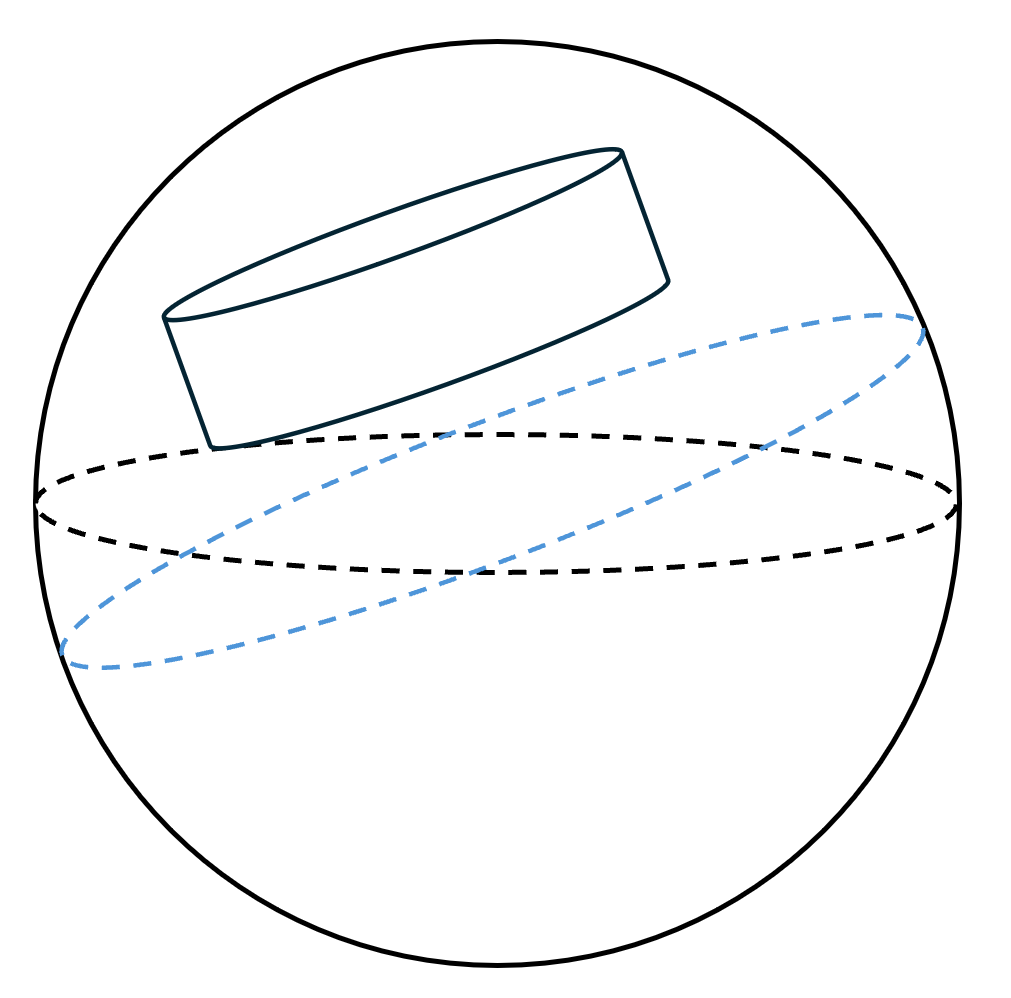
\includegraphics[width=0.25\linewidth]{figures/Figure1.png}
    \caption{Situation (1)}
\end{figure}

\begin{figure}
    \centering
    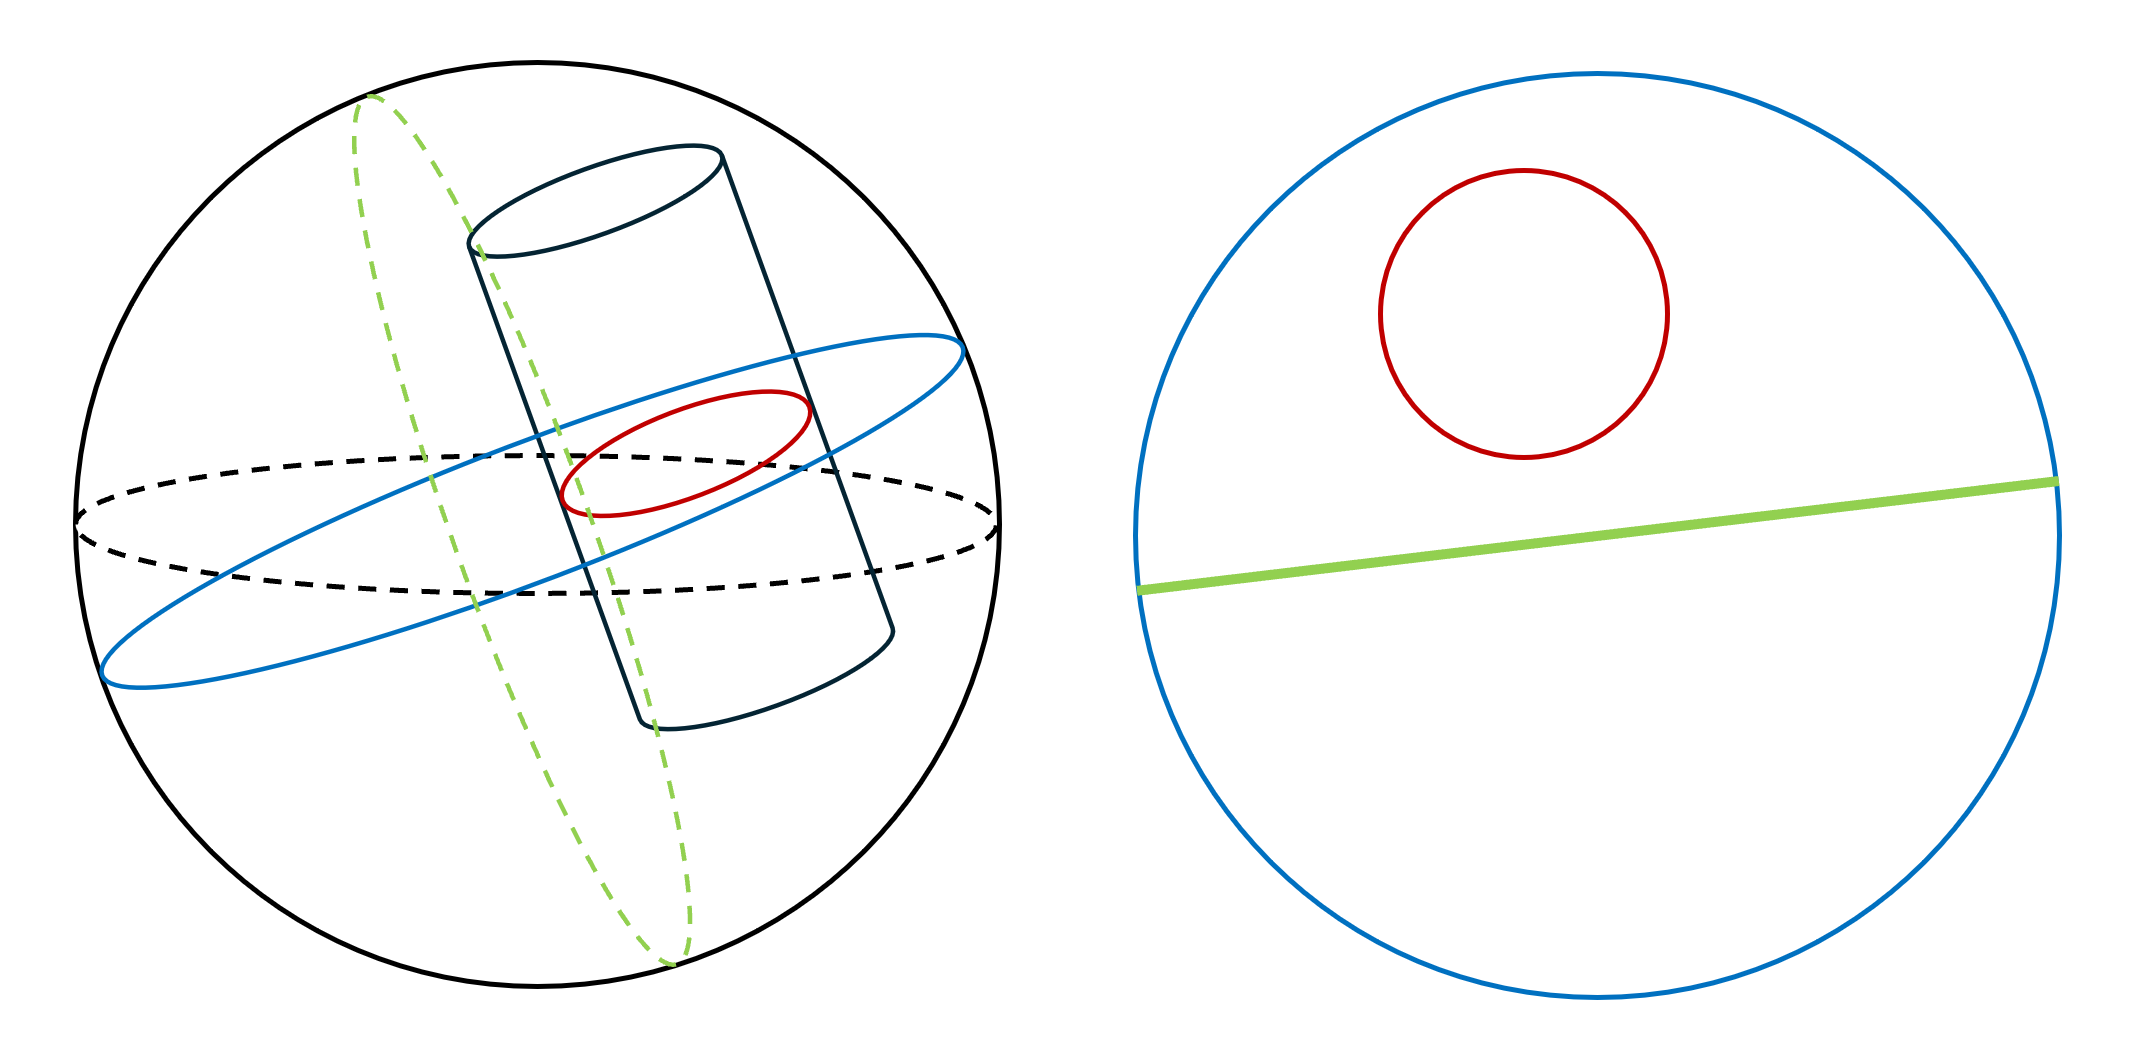
\includegraphics[width=0.5\linewidth]{figures/Figure2.png}
    \caption{Situation (2)}
\end{figure}

\end{answer}



\begin{problem}{8 (20')} 
Consider the following geometries in $d$-dimensional space:
\begin{align*}
    \Phi_d=\left\{(x_1,\cdots,x_d)\mid x_1^2+\cdots+x_d^2\leq 1\right\}\qquad
    \Omega_d=\left\{(x_1,\cdots,x_d)\mid |x_1|+\cdots+|x_d|\leq 1\right\}
\end{align*}
\begin{itemize}
    \item [(1)] (6') Consider the following two random processes:
    \begin{itemize}
        \item Pick two uniformly random unit vectors $x,y$ from the sphere in $d$ dimension.
        \item Pick a uniformly random plane passing through the origin in $d$ dimensions. Then pick two uniformly random unit vectors $w,z$ from the 2D sphere lying on that plane.
    \end{itemize}
    Determine whether $x$ and $w$ are identically distributed, and whether the pairs $(x,y)$ and $(w,z)$ are identically distributed. Briefly explain the reasons.
    \item [(2)] (6') Suppose $x$ and $y$ are sampled independently from $\Phi_d$. Denote random variable $Z=x^\top y$. Calculate $Var(Z)$.
    \item [(3)] (8') Calculate $V(\Omega_d)$ (the volume of $\Omega_d$) and $A(\Omega_d)$ (the surface area of $\Omega_d$).
\end{itemize}
\end{problem}

\begin{answer} ~
\begin{itemize}
    \item [(1)] $x$ and $w$ is identically distributed since they are both uniformly random unit vectors from the sphere. But $(x,y)$ and $(w,z)$ is not: consider their inner product, the inner product of $w$ and $z$ is always the distribution on 2D sphere, which is different with high-dimensional inner product distribution.
    \item [(2)] For any $i$, $\E(x_i) = 0$, $\E(y_i) = 0$. According to symmetry, for any $i \neq j$, $\E(x_ix_j) = \E(-x_ix_j) = -\E(x_ix_j)$, so $\E(x_ix_j) = 0$. According to Problem 5, for any $i$, $\E(x_i^2) = \frac{1}{d+2}$. Then,
    \[\begin{aligned}
    Var(x^\top y) &= \E((x^\top y)^2) - (\E(x^\top y))^2 \\
    &= \E\left(\sum_{i,j} x_iy_ix_jy_j\right) - \left(\E\left(\sum_i x_iy_i\right)\right)^2 \\
    &= \sum_{i.j}\E(x_ix_j)\E(y_iy_j) - \left(\sum_i \E(x_i)\E(y_i)\right)^2 \\
    &= \sum_i \E(x_i^2)\E(y_i^2) \\
    &= \frac{d}{(d+2)^2}
    \end{aligned}\]
    \item [(3)] First calculate the volume. Fix $x_1$, then $|x_2| + \dots + |x_d| \le 1 - |x_1|$. Use $\Omega_{d, r}$ to represent the geometry of $|x_1| + \dots + |x_d| \le r$, then:
    \[\begin{aligned}
    V(\Omega_d) &= \int_{-1}^1 V(\Omega_{d-1, 1-|x_1|}) \dd x_1 \\
    &= V(\Omega_{d-1}) \int_{-1}^1 (1-|x_1|)^{d-1} \dd x_1 \\
    &= 2V(\Omega_{d-1}) \int_0^1 (1-x_1)^{d-1} \dd x_1 \\
    &= \frac{2}{d} V(\Omega_{d-1}) \\
    &= \dots \\
    &= \frac{2^{d-1}}{d!} V(\Omega_{1}) \\
    &= \frac{2^d}{d!}
    \end{aligned}\]
    Then, by the co-area formula(Let $f(x) = |x_1| + \dots + |x_d|$, then $|\nabla f(x)| = \sqrt{d}$)
    \[\begin{aligned}
    V(\Omega_d) &= \int_0^1 \frac{A(\Omega_{d,r})}{\sqrt{d}} \dd r \\
    &= \frac{A(\Omega_d)}{\sqrt{d}} \int_0^1 r^{d-1} \dd r \\
    &= \frac{A(\Omega_d)}{d\sqrt{d}}
    \end{aligned}\]
    As a result,
    \[
    A(\Omega_d) = d\sqrt{d}V(\Omega_d) = \frac{2^d\sqrt{d}}{(d-1)!}
    \]
\end{itemize}
\end{answer}



\end{document}